\question
Булева функция задана диаграммой Эйлера-Венна. Задайте данную функцию формулой, используя только опреации XOR, NAND, NOR. Изобразите её в виде функциональной схемы.

\begin{figure}[h]

\begin{minipage}[h]{0.55\linewidth}
\end{minipage}
\begin{minipage}[h]{0.45\linewidth}
\center{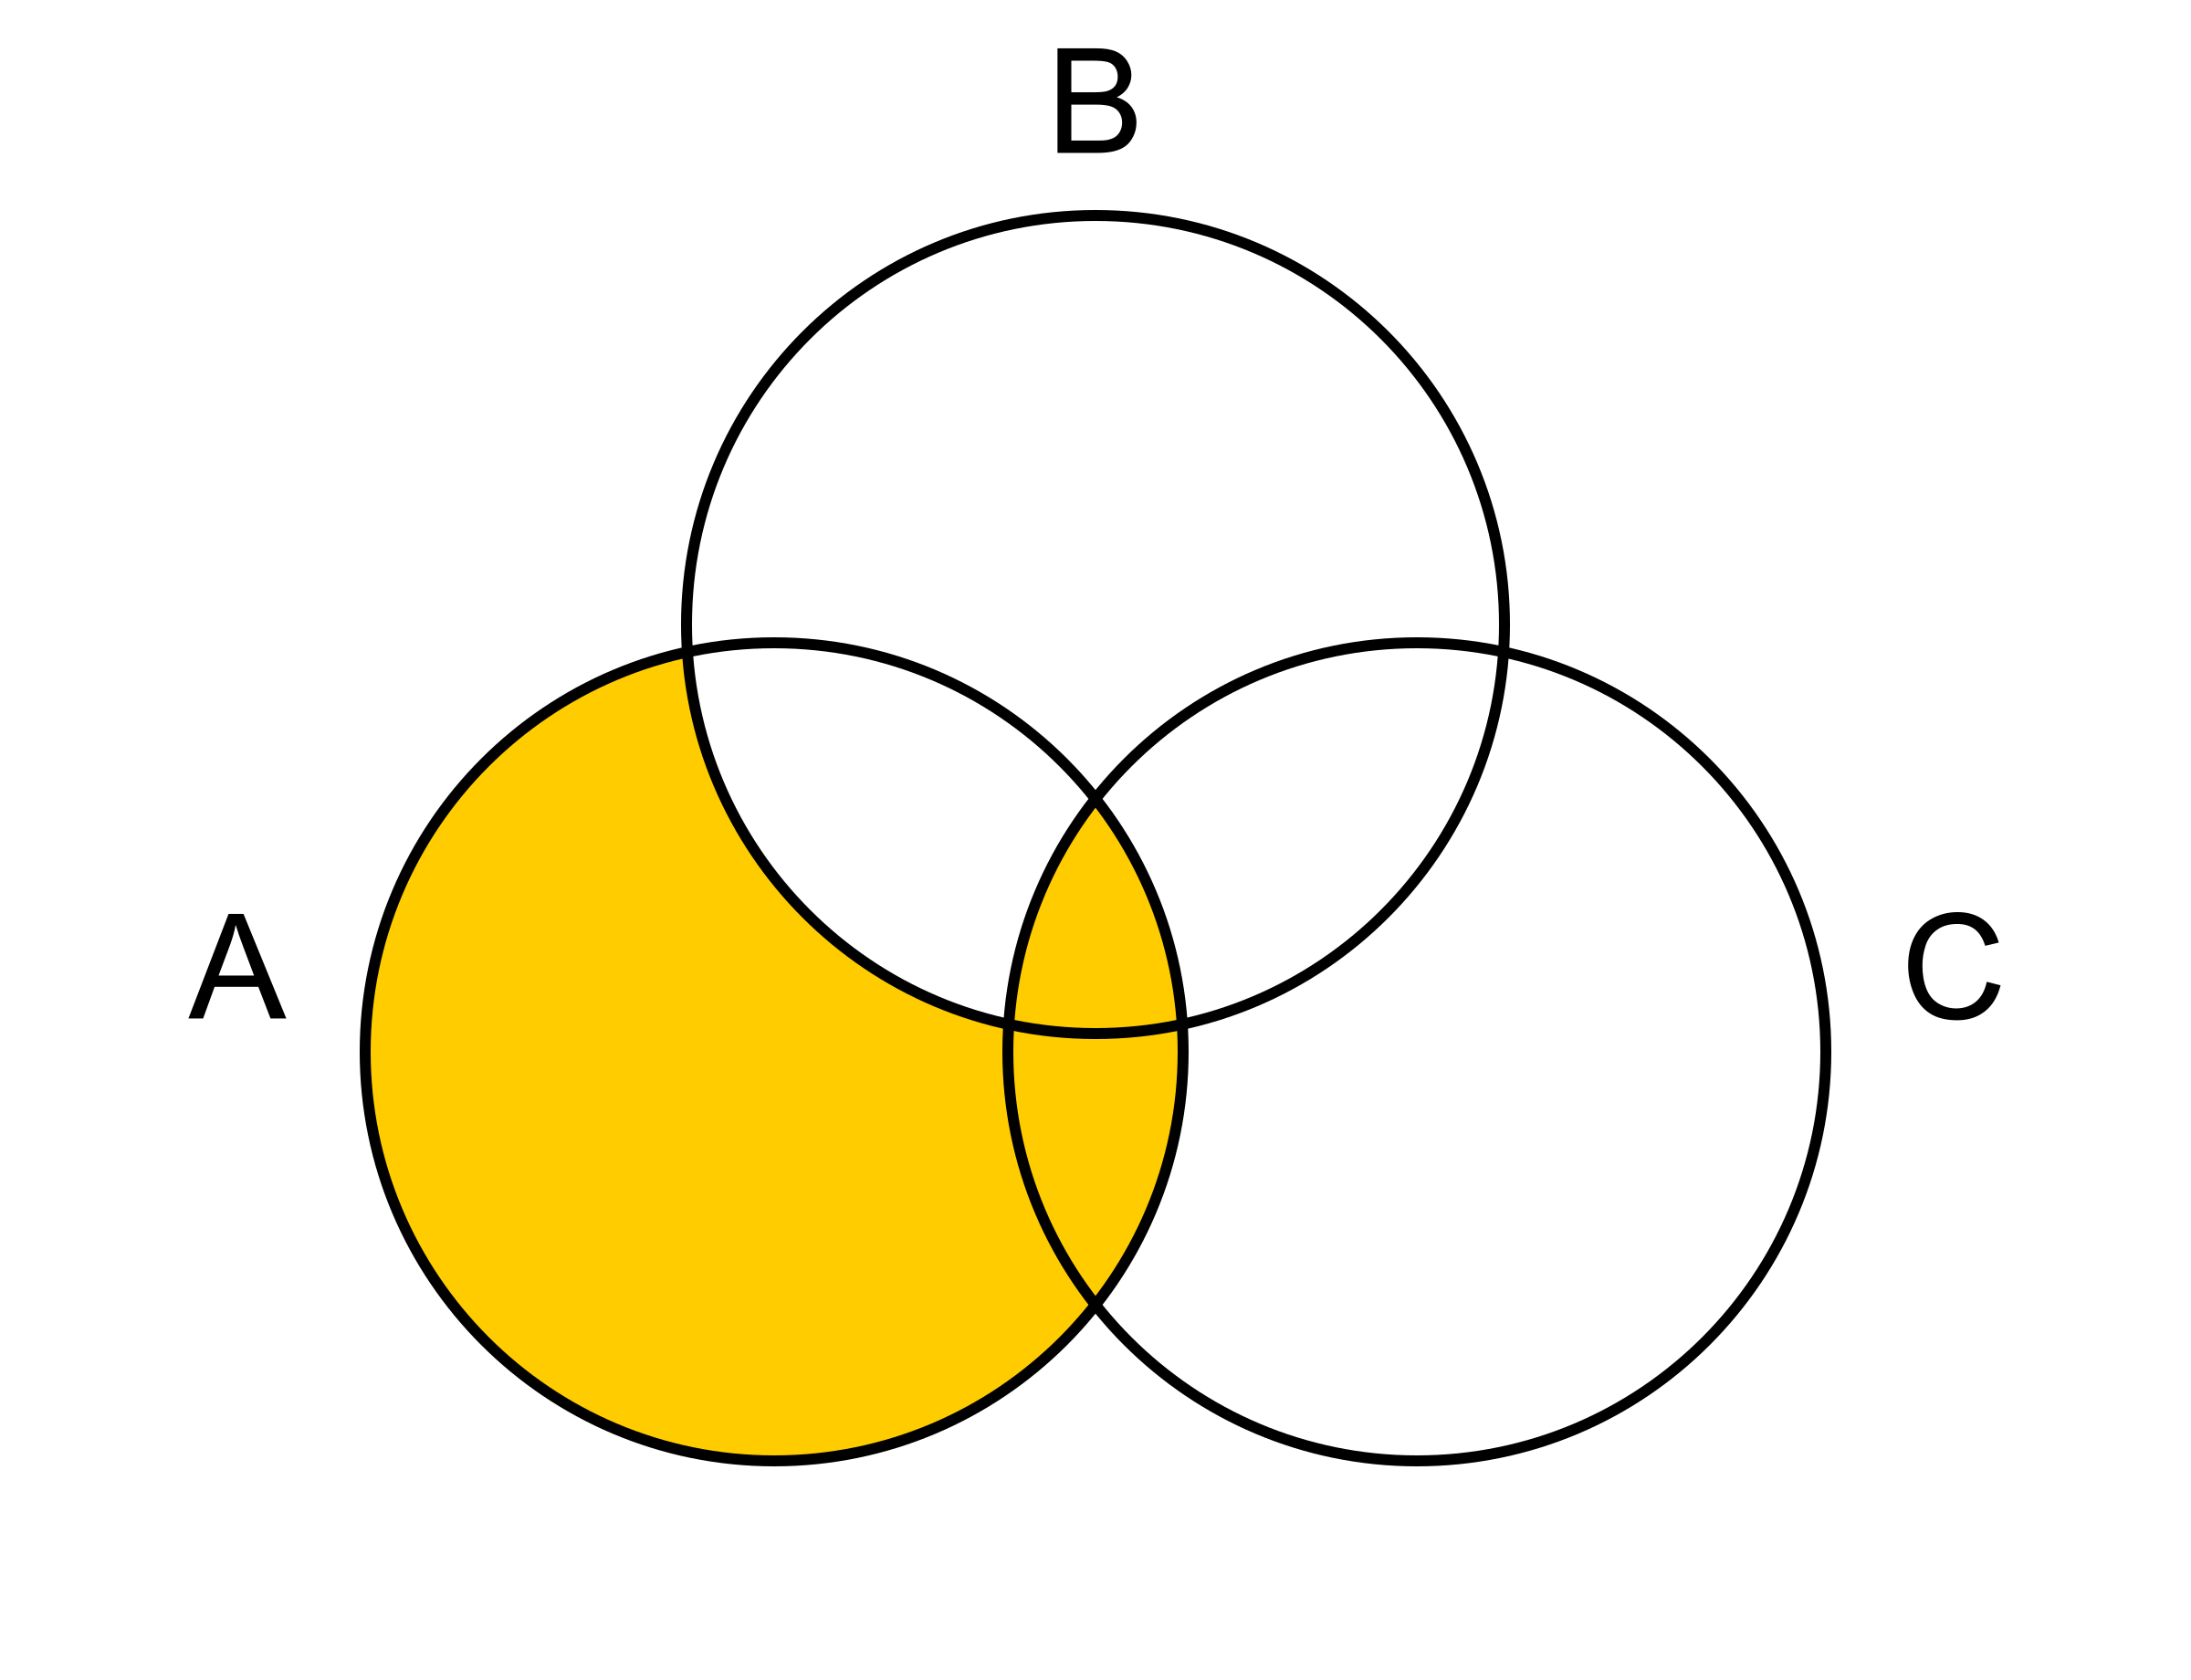
\includegraphics[width=0.7\textwidth]{pic/871.png} }
\end{minipage}
\end{figure}

---------------

Автор -- Марат Ибрагимов